% Options for packages loaded elsewhere
\PassOptionsToPackage{unicode}{hyperref}
\PassOptionsToPackage{hyphens}{url}
\documentclass[
  11pt,
]{article}
\usepackage{xcolor}
\usepackage[margin=1in]{geometry}
\usepackage{amsmath,amssymb}
\setcounter{secnumdepth}{5}
\usepackage{iftex}
\ifPDFTeX
  \usepackage[T1]{fontenc}
  \usepackage[utf8]{inputenc}
  \usepackage{textcomp} % provide euro and other symbols
\else % if luatex or xetex
  \usepackage{unicode-math} % this also loads fontspec
  \defaultfontfeatures{Scale=MatchLowercase}
  \defaultfontfeatures[\rmfamily]{Ligatures=TeX,Scale=1}
\fi
\usepackage{lmodern}
\ifPDFTeX\else
  % xetex/luatex font selection
\fi
% Use upquote if available, for straight quotes in verbatim environments
\IfFileExists{upquote.sty}{\usepackage{upquote}}{}
\IfFileExists{microtype.sty}{% use microtype if available
  \usepackage[]{microtype}
  \UseMicrotypeSet[protrusion]{basicmath} % disable protrusion for tt fonts
}{}
\makeatletter
\@ifundefined{KOMAClassName}{% if non-KOMA class
  \IfFileExists{parskip.sty}{%
    \usepackage{parskip}
  }{% else
    \setlength{\parindent}{0pt}
    \setlength{\parskip}{6pt plus 2pt minus 1pt}}
}{% if KOMA class
  \KOMAoptions{parskip=half}}
\makeatother
\usepackage{color}
\usepackage{fancyvrb}
\newcommand{\VerbBar}{|}
\newcommand{\VERB}{\Verb[commandchars=\\\{\}]}
\DefineVerbatimEnvironment{Highlighting}{Verbatim}{commandchars=\\\{\}}
% Add ',fontsize=\small' for more characters per line
\usepackage{framed}
\definecolor{shadecolor}{RGB}{248,248,248}
\newenvironment{Shaded}{\begin{snugshade}}{\end{snugshade}}
\newcommand{\AlertTok}[1]{\textcolor[rgb]{0.94,0.16,0.16}{#1}}
\newcommand{\AnnotationTok}[1]{\textcolor[rgb]{0.56,0.35,0.01}{\textbf{\textit{#1}}}}
\newcommand{\AttributeTok}[1]{\textcolor[rgb]{0.13,0.29,0.53}{#1}}
\newcommand{\BaseNTok}[1]{\textcolor[rgb]{0.00,0.00,0.81}{#1}}
\newcommand{\BuiltInTok}[1]{#1}
\newcommand{\CharTok}[1]{\textcolor[rgb]{0.31,0.60,0.02}{#1}}
\newcommand{\CommentTok}[1]{\textcolor[rgb]{0.56,0.35,0.01}{\textit{#1}}}
\newcommand{\CommentVarTok}[1]{\textcolor[rgb]{0.56,0.35,0.01}{\textbf{\textit{#1}}}}
\newcommand{\ConstantTok}[1]{\textcolor[rgb]{0.56,0.35,0.01}{#1}}
\newcommand{\ControlFlowTok}[1]{\textcolor[rgb]{0.13,0.29,0.53}{\textbf{#1}}}
\newcommand{\DataTypeTok}[1]{\textcolor[rgb]{0.13,0.29,0.53}{#1}}
\newcommand{\DecValTok}[1]{\textcolor[rgb]{0.00,0.00,0.81}{#1}}
\newcommand{\DocumentationTok}[1]{\textcolor[rgb]{0.56,0.35,0.01}{\textbf{\textit{#1}}}}
\newcommand{\ErrorTok}[1]{\textcolor[rgb]{0.64,0.00,0.00}{\textbf{#1}}}
\newcommand{\ExtensionTok}[1]{#1}
\newcommand{\FloatTok}[1]{\textcolor[rgb]{0.00,0.00,0.81}{#1}}
\newcommand{\FunctionTok}[1]{\textcolor[rgb]{0.13,0.29,0.53}{\textbf{#1}}}
\newcommand{\ImportTok}[1]{#1}
\newcommand{\InformationTok}[1]{\textcolor[rgb]{0.56,0.35,0.01}{\textbf{\textit{#1}}}}
\newcommand{\KeywordTok}[1]{\textcolor[rgb]{0.13,0.29,0.53}{\textbf{#1}}}
\newcommand{\NormalTok}[1]{#1}
\newcommand{\OperatorTok}[1]{\textcolor[rgb]{0.81,0.36,0.00}{\textbf{#1}}}
\newcommand{\OtherTok}[1]{\textcolor[rgb]{0.56,0.35,0.01}{#1}}
\newcommand{\PreprocessorTok}[1]{\textcolor[rgb]{0.56,0.35,0.01}{\textit{#1}}}
\newcommand{\RegionMarkerTok}[1]{#1}
\newcommand{\SpecialCharTok}[1]{\textcolor[rgb]{0.81,0.36,0.00}{\textbf{#1}}}
\newcommand{\SpecialStringTok}[1]{\textcolor[rgb]{0.31,0.60,0.02}{#1}}
\newcommand{\StringTok}[1]{\textcolor[rgb]{0.31,0.60,0.02}{#1}}
\newcommand{\VariableTok}[1]{\textcolor[rgb]{0.00,0.00,0.00}{#1}}
\newcommand{\VerbatimStringTok}[1]{\textcolor[rgb]{0.31,0.60,0.02}{#1}}
\newcommand{\WarningTok}[1]{\textcolor[rgb]{0.56,0.35,0.01}{\textbf{\textit{#1}}}}
\usepackage{longtable,booktabs,array}
\newcounter{none} % for unnumbered tables
\usepackage{calc} % for calculating minipage widths
% Correct order of tables after \paragraph or \subparagraph
\usepackage{etoolbox}
\makeatletter
\patchcmd\longtable{\par}{\if@noskipsec\mbox{}\fi\par}{}{}
\makeatother
% Allow footnotes in longtable head/foot
\IfFileExists{footnotehyper.sty}{\usepackage{footnotehyper}}{\usepackage{footnote}}
\makesavenoteenv{longtable}
\usepackage{graphicx}
\makeatletter
\newsavebox\pandoc@box
\newcommand*\pandocbounded[1]{% scales image to fit in text height/width
  \sbox\pandoc@box{#1}%
  \Gscale@div\@tempa{\textheight}{\dimexpr\ht\pandoc@box+\dp\pandoc@box\relax}%
  \Gscale@div\@tempb{\linewidth}{\wd\pandoc@box}%
  \ifdim\@tempb\p@<\@tempa\p@\let\@tempa\@tempb\fi% select the smaller of both
  \ifdim\@tempa\p@<\p@\scalebox{\@tempa}{\usebox\pandoc@box}%
  \else\usebox{\pandoc@box}%
  \fi%
}
% Set default figure placement to htbp
\def\fps@figure{htbp}
\makeatother
\setlength{\emergencystretch}{3em} % prevent overfull lines
\providecommand{\tightlist}{%
  \setlength{\itemsep}{0pt}\setlength{\parskip}{0pt}}
\usepackage{booktabs}
\usepackage{float}
\usepackage{booktabs}
\usepackage{longtable}
\usepackage{array}
\usepackage{multirow}
\usepackage{wrapfig}
\usepackage{float}
\usepackage{colortbl}
\usepackage{pdflscape}
\usepackage{tabu}
\usepackage{threeparttable}
\usepackage{threeparttablex}
\usepackage[normalem]{ulem}
\usepackage{makecell}
\usepackage{xcolor}
\usepackage{bookmark}
\IfFileExists{xurl.sty}{\usepackage{xurl}}{} % add URL line breaks if available
\urlstyle{same}
\hypersetup{
  pdftitle={Multivariate Comparison of Two Biting-Fly Species},
  pdfauthor={Author 1 \& Author 2},
  hidelinks,
  pdfcreator={LaTeX via pandoc}}

\title{Multivariate Comparison of Two Biting-Fly Species}
\usepackage{etoolbox}
\makeatletter
\providecommand{\subtitle}[1]{% add subtitle to \maketitle
  \apptocmd{\@title}{\par {\large #1 \par}}{}{}
}
\makeatother
\subtitle{Statistics 232C - Midterm Take-home, Spring 2025}
\author{Author 1 \& Author 2}
\date{May 08, 2026}

\begin{document}
\maketitle

{
\setcounter{tocdepth}{3}
\tableofcontents
}
\section{Introduction}\label{introduction}

Two species of biting flies of the genus \emph{Leptoconops} --- \emph{L.
torrens} and \emph{L. carteri} --- are nearly indistinguishable in
external morphology and were long believed to be a single species.
Subsequent biological studies revealed differences in sex ratio at
emergence and in biting behaviour. The data set \texttt{flies.xls}
records seven morphometric measurements taken on 35 flies of each
species (total \(n = 70\)). The aim of this analysis is to determine,
using multivariate statistical methodology, whether the two populations
differ and, if so, on which morphological characters.

The seven measured variables are:

{\def\LTcaptype{none} % do not increment counter
\begin{longtable}[]{@{}lll@{}}
\toprule\noalign{}
Code & Variable & Meaning \\
\midrule\noalign{}
\endhead
\bottomrule\noalign{}
\endlastfoot
\(X_1\) & \texttt{W\_len} & Wing length \\
\(X_2\) & \texttt{W\_wid} & Wing width \\
\(X_3\) & \texttt{P3\_len} & Third-palp length \\
\(X_4\) & \texttt{P3\_wid} & Third-palp width \\
\(X_5\) & \texttt{P4\_len} & Fourth-palp length \\
\(X_6\) & \texttt{Ant12} & Length of antennal segment 12 \\
\(X_7\) & \texttt{Ant13} & Length of antennal segment 13 \\
\end{longtable}
}

The response indicator \texttt{Species} equals 0 for \emph{L. torrens}
and 1 for \emph{L. carteri}.

\section{Data}\label{data}

\begin{verbatim}
## Rows: 70
## Columns: 8
## $ W_len   <dbl> 85, 87, 94, 92, 96, 91, 90, 92, 91, 87, 97, 89, 94, 96, 104, 9~
## $ W_wid   <dbl> 41, 38, 44, 43, 43, 44, 42, 43, 41, 38, 45, 38, 45, 44, 49, 41~
## $ P3_len  <dbl> 31, 32, 36, 32, 35, 36, 36, 36, 36, 35, 39, 36, 37, 37, 35, 31~
## $ P3_wid  <dbl> 13, 14, 15, 17, 14, 12, 16, 17, 14, 11, 17, 13, 13, 14, 14, 17~
## $ P4_len  <dbl> 25, 22, 27, 28, 26, 24, 26, 26, 23, 24, 27, 22, 26, 24, 21, 26~
## $ Ant12   <dbl> 9, 13, 8, 9, 10, 9, 9, 9, 9, 9, 9, 9, 9, 9, 10, 10, 10, 9, 9, ~
## $ Ant13   <dbl> 8, 13, 9, 9, 10, 9, 9, 9, 9, 10, 10, 9, 9, 10, 10, 9, 9, 9, 10~
## $ Species <fct> L.torrens, L.torrens, L.torrens, L.torrens, L.torrens, L.torre~
\end{verbatim}

\subsection{Descriptive statistics}\label{descriptive-statistics}

\begin{longtable}[t]{lrrrrr}
\caption{\label{tab:desc-tbl}Per-species means and standard deviations.}\\
\toprule
Variable & Mean\_L.torrens & Mean\_L.carteri & SD\_L.torrens & SD\_L.carteri & Diff\\
\midrule
Ant12 & 9.57 & 9.66 & 0.92 & 1.26 & -0.09\\
Ant13 & 9.71 & 9.37 & 0.89 & 1.09 & 0.34\\
P3\_len & 35.37 & 39.31 & 2.20 & 2.84 & -3.94\\
P3\_wid & 14.51 & 14.66 & 1.84 & 1.64 & -0.14\\
P4\_len & 25.63 & 30.00 & 2.50 & 4.61 & -4.37\\
\addlinespace
W\_len & 96.46 & 99.34 & 6.38 & 5.59 & -2.89\\
W\_wid & 42.91 & 43.74 & 2.74 & 5.08 & -0.83\\
\bottomrule
\end{longtable}

\begin{figure}

{\centering 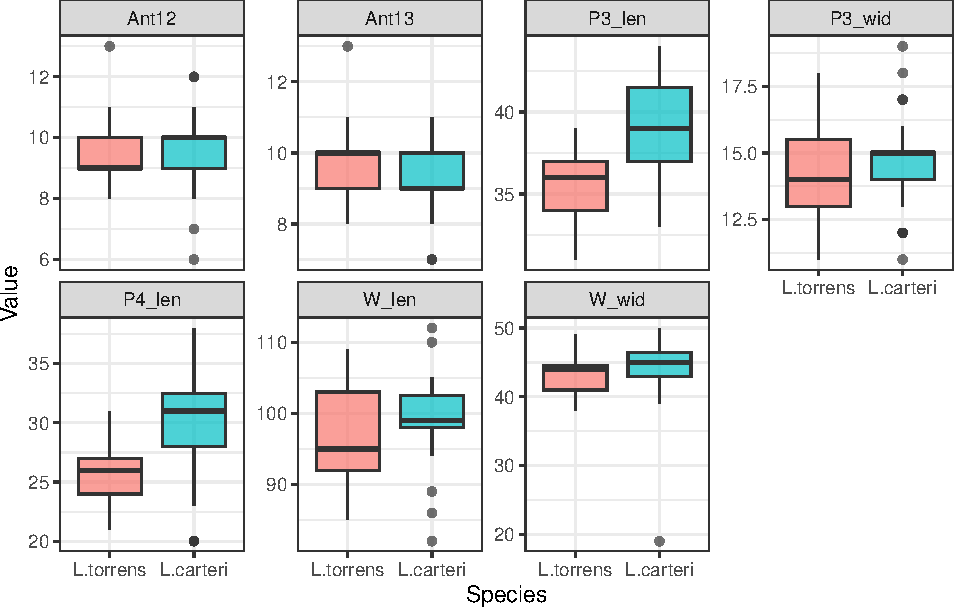
\includegraphics[width=0.85\linewidth]{Midterm_Report_files/figure-latex/boxplot-1} 

}

\caption{Side-by-side boxplots of the seven variables.}\label{fig:boxplot}
\end{figure}

\begin{figure}

{\centering 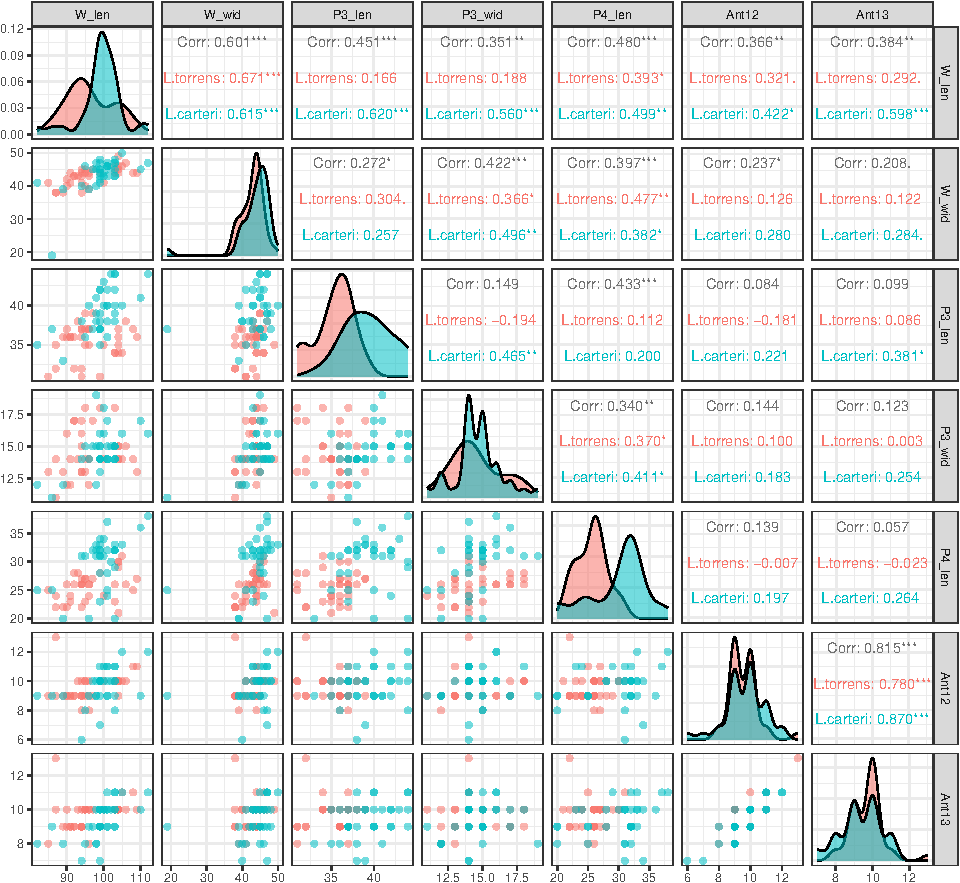
\includegraphics[width=0.85\linewidth]{Midterm_Report_files/figure-latex/pairs-1} 

}

\caption{Pair-wise scatter plot matrix coloured by species.}\label{fig:pairs}
\end{figure}

\section{Normality assessment}\label{normality-assessment}

\subsection{Univariate Q--Q plots and Shapiro--Wilk
tests}\label{univariate-qq-plots-and-shapirowilk-tests}

\begin{figure}

{\centering 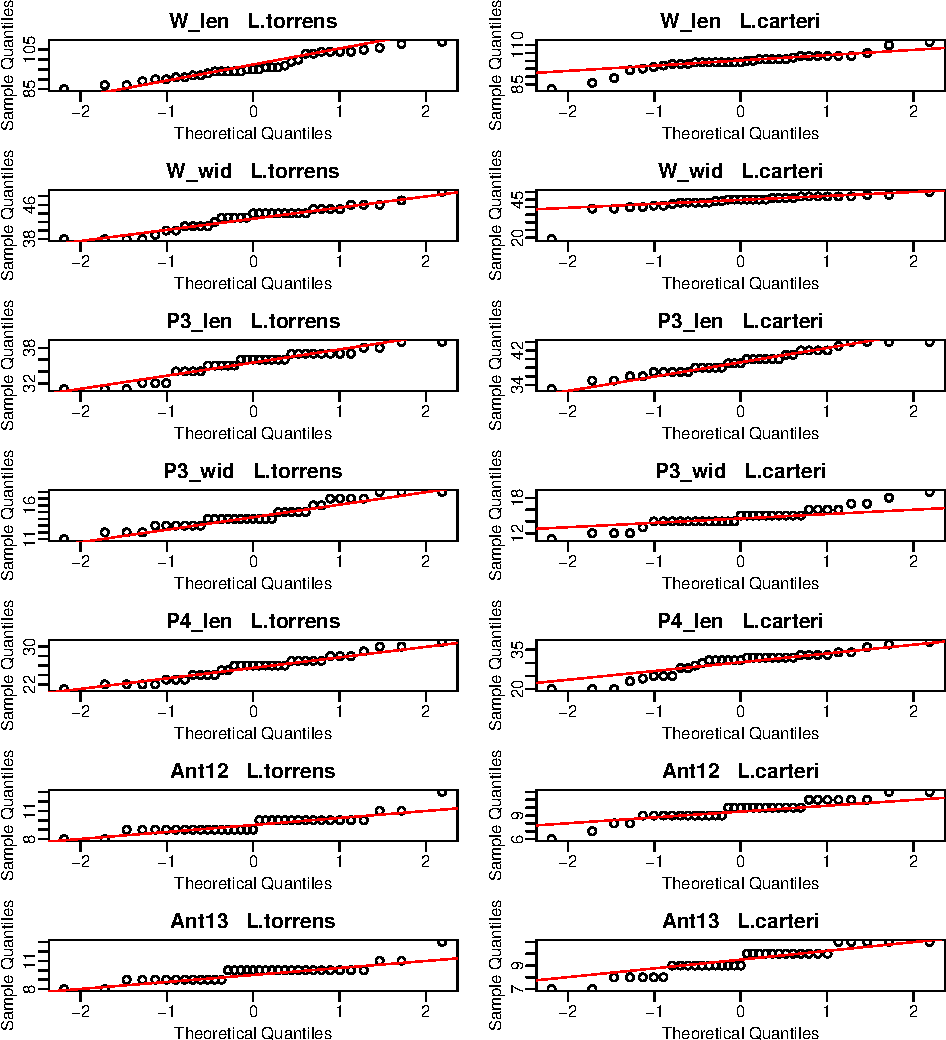
\includegraphics[width=0.85\linewidth]{Midterm_Report_files/figure-latex/qq-univ-1} 

}

\caption{Normal Q–Q plots for each variable, by species.}\label{fig:qq-univ}
\end{figure}

\begin{longtable}[t]{lrr}
\caption{\label{tab:shapiro}Shapiro–Wilk p-values (variables in rows).}\\
\toprule
 & L.torrens & L.carteri\\
\midrule
W\_len & 0.122 & 0.002\\
W\_wid & 0.077 & 0.000\\
P3\_len & 0.015 & 0.351\\
P3\_wid & 0.034 & 0.038\\
P4\_len & 0.304 & 0.004\\
\addlinespace
Ant12 & 0.000 & 0.013\\
Ant13 & 0.000 & 0.007\\
\bottomrule
\end{longtable}

\subsection{Multivariate normality}\label{multivariate-normality}

\begin{longtable}[t]{lrrrl}
\caption{\label{tab:mvn}Mardia test of multivariate normality, L. torrens.}\\
\toprule
Test & Statistic & df & p\_value & Reject\_H0\\
\midrule
Mardia skewness & 159.538 & 84 & 1.30e-06 & Yes\\
Mardia kurtosis & 2.131 & NA & 3.31e-02 & Yes\\
\bottomrule
\end{longtable}

\begin{longtable}[t]{lrrrl}
\caption{\label{tab:mvn}Mardia test of multivariate normality, L. carteri.}\\
\toprule
Test & Statistic & df & p\_value & Reject\_H0\\
\midrule
Mardia skewness & 158.437 & 84 & 1.70e-06 & Yes\\
Mardia kurtosis & 2.861 & NA & 4.22e-03 & Yes\\
\bottomrule
\end{longtable}

\begin{figure}

{\centering 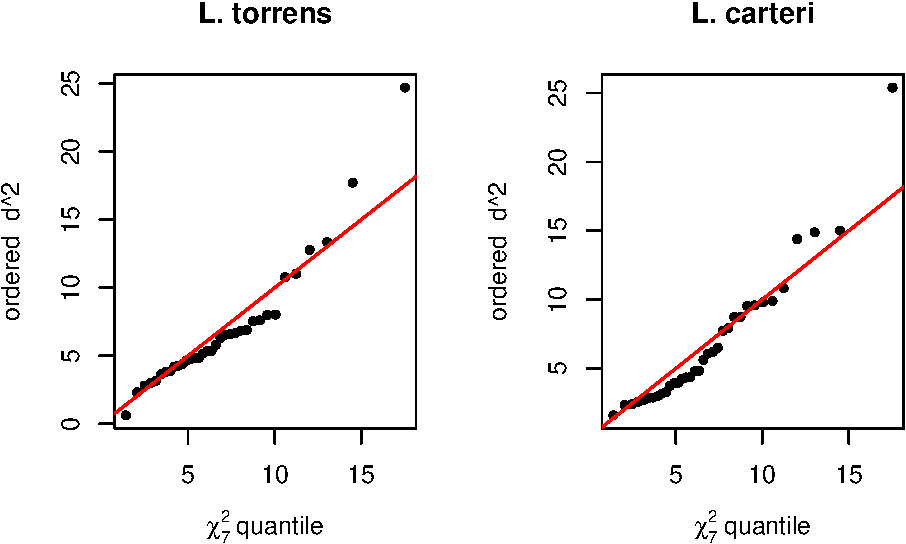
\includegraphics[width=0.85\linewidth]{Midterm_Report_files/figure-latex/chisq-qq-1} 

}

\caption{Chi-squared Q–Q plots of squared Mahalanobis distances.}\label{fig:chisq-qq}
\end{figure}

\section{Outlier detection}\label{outlier-detection}

\begin{longtable}[t]{llrrl}
\caption{\label{tab:outliers}Cases with $d^2 > 16.01$.}\\
\toprule
 & Species & Index & D2 & Outlier\\
\midrule
2 & L.torrens & 2 & 24.70 & TRUE\\
15 & L.torrens & 15 & 17.72 & TRUE\\
36 & L.carteri & 1 & 25.38 & TRUE\\
\bottomrule
\end{longtable}

\section{Transformations}\label{transformations}

To stabilise variance and improve approximate joint normality, we
estimated the optimal Box-Cox parameter \(\lambda\) separately for each
of the seven morphometric variables (using the pooled sample, so the
same \(\lambda\) is applied to both species and the variables remain on
comparable scales).

\begin{longtable}[t]{rrrrrrr}
\caption{\label{tab:lambda-tbl}Optimal Box-Cox lambdas (per variable).}\\
\toprule
W\_len & W\_wid & P3\_len & P3\_wid & P4\_len & Ant12 & Ant13\\
\midrule
2 & 2 & 0.1 & 0 & 0.4 & 1.1 & 1\\
\bottomrule
\end{longtable}

The estimated \(\lambda\) values are heterogeneous: the wing dimensions
favour a power-2 transformation, the third-palp variables favour log
(\(\lambda \approx 0\)), the fourth-palp length is closest to a square
root (\(\lambda \approx 0.5\)), while the antennal segments are
essentially linear (\(\lambda \approx 1\)). A single uniform
transformation (e.g.~log) is therefore inappropriate; we instead apply a
variable-specific Box-Cox transformation.

\begin{longtable}[t]{lrrrl}
\caption{\label{tab:bctrans}Mardia test after variable-specific Box-Cox, L. torrens.}\\
\toprule
Test & Statistic & df & p\_value & Reject\_H0\\
\midrule
Mardia skewness & 162.672 & 84 & 6.00e-07 & Yes\\
Mardia kurtosis & 2.316 & NA & 2.06e-02 & Yes\\
\bottomrule
\end{longtable}

\begin{longtable}[t]{lrrrl}
\caption{\label{tab:bctrans}Mardia test after variable-specific Box-Cox, L. carteri.}\\
\toprule
Test & Statistic & df & p\_value & Reject\_H0\\
\midrule
Mardia skewness & 119.416 & 84 & 0.00672 & Yes\\
Mardia kurtosis & 1.528 & NA & 0.12600 & No\\
\bottomrule
\end{longtable}

\begin{figure}

{\centering 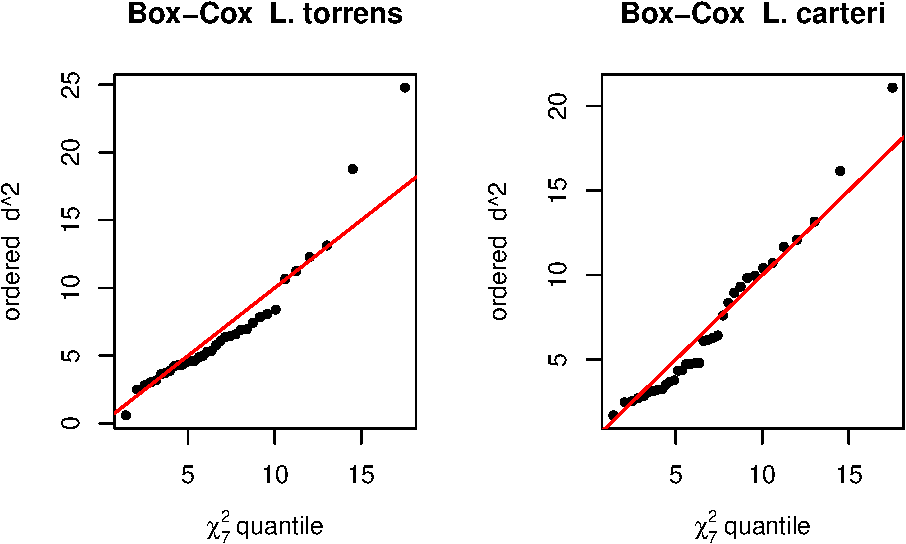
\includegraphics[width=0.85\linewidth]{Midterm_Report_files/figure-latex/chisq-qq-bc-1} 

}

\caption{Chi-squared Q-Q plots after variable-specific Box-Cox transformation.}\label{fig:chisq-qq-bc}
\end{figure}

\begin{longtable}[t]{llrrl}
\caption{\label{tab:outliers-bc}Cases with $d^2 > 16.01$ after Box-Cox transformation.}\\
\toprule
 & Species & Index & D2 & Outlier\\
\midrule
2 & L.torrens & 2 & 24.78 & TRUE\\
15 & L.torrens & 15 & 18.77 & TRUE\\
36 & L.carteri & 1 & 21.10 & TRUE\\
51 & L.carteri & 16 & 16.16 & TRUE\\
\bottomrule
\end{longtable}

\subsection{Sensitivity analysis: outlier
removal}\label{sensitivity-analysis-outlier-removal}

Mardia's tests on the full sample still flag departures from joint
normality, partly because the test is conservative when \(n\) is below
the \(p(p+1)(p+2)/6 = 84\) threshold and partly because a few
high-\(d^2\) observations inflate the skewness statistic. As a
sensitivity check we remove cases whose squared Mahalanobis distance on
the \textbf{raw} scale exceeded the \(\chi^2_{7,0.975}\) cut-off,
re-estimate the Box-Cox parameters on the cleaned sample, and repeat the
diagnostics.

\begin{longtable}[t]{lrrrrrrr}
\caption{\label{tab:lambda-clean-tbl}Optimal Box-Cox lambdas, before vs. after outlier removal.}\\
\toprule
 & W\_len & W\_wid & P3\_len & P3\_wid & P4\_len & Ant12 & Ant13\\
\midrule
Full sample & 2 & 2 & 0.1 & 0.0 & 0.4 & 1.1 & 1\\
Outliers removed & 2 & 2 & 0.3 & -0.2 & 0.6 & 1.9 & 2\\
\bottomrule
\end{longtable}

\begin{longtable}[t]{lrrrl}
\caption{\label{tab:mardia-clean}Mardia test after Box-Cox + outlier removal, L. torrens (n = 33).}\\
\toprule
Test & Statistic & df & p\_value & Reject\_H0\\
\midrule
Mardia skewness & 100.908 & 84 & 0.101 & No\\
Mardia kurtosis & -0.476 & NA & 0.634 & No\\
\bottomrule
\end{longtable}

\begin{longtable}[t]{lrrrl}
\caption{\label{tab:mardia-clean}Mardia test after Box-Cox + outlier removal, L. carteri (n = 34).}\\
\toprule
Test & Statistic & df & p\_value & Reject\_H0\\
\midrule
Mardia skewness & 81.236 & 84 & 0.565 & No\\
Mardia kurtosis & -0.110 & NA & 0.912 & No\\
\bottomrule
\end{longtable}

\begin{figure}

{\centering 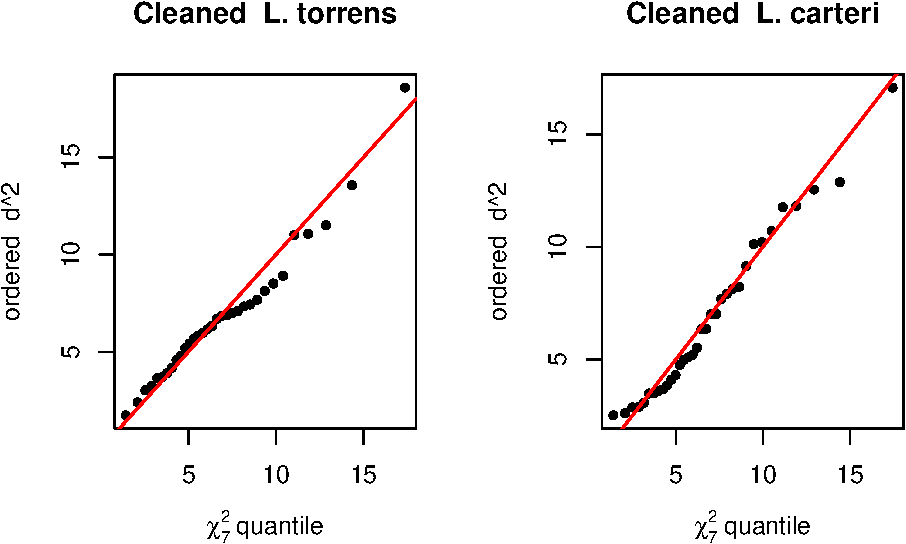
\includegraphics[width=0.85\linewidth]{Midterm_Report_files/figure-latex/chisq-qq-clean-1} 

}

\caption{Chi-squared Q-Q plots after Box-Cox + outlier removal.}\label{fig:chisq-qq-clean}
\end{figure}

If the cleaned-sample Mardia tests no longer reject (or reject with
substantially larger p-values), we treat the multivariate-normality
assumption as adequately satisfied and use the cleaned, transformed data
as the basis of the inferential analysis below; the full-sample analysis
is reported alongside as a robustness check.

\section{Equality of covariance
matrices}\label{equality-of-covariance-matrices}

\begin{verbatim}
## $raw
## 
##  Box's M-test for Homogeneity of Covariance Matrices
## 
## data:  X
## Chi-Sq (approx.) = 64.539, df = 28, p-value = 0.0001039
## 
## 
## $box_cox
## 
##  Box's M-test for Homogeneity of Covariance Matrices
## 
## data:  Xbc
## Chi-Sq (approx.) = 54.339, df = 28, p-value = 0.00204
## 
## 
## $box_cox_clean
## 
##  Box's M-test for Homogeneity of Covariance Matrices
## 
## data:  Xbc_c
## Chi-Sq (approx.) = 67.012, df = 28, p-value = 4.813e-05
\end{verbatim}

If Box's \(M\) does not reject equality of covariances on the
transformed scale, the standard pooled-covariance Hotelling \(T^2\) is
appropriate; otherwise a James / Yao correction would be more
conservative. We report both raw- and transformed-scale results.

\section{\texorpdfstring{Hotelling's \(T^2\)
test}{Hotelling's T\^{}2 test}}\label{hotellings-t2-test}

\begin{verbatim}
## 
##  Hotelling's two sample T2-test
## 
## data:  X1 and X2
## T.2 = 13.824, df1 = 7, df2 = 62, p-value = 1.233e-10
## alternative hypothesis: true location difference is not equal to c(0,0,0,0,0,0,0)
\end{verbatim}

\begin{verbatim}
## 
##  Hotelling's two sample T2-test
## 
## data:  X1bc and X2bc
## T.2 = 13.145, df1 = 7, df2 = 62, p-value = 3.016e-10
## alternative hypothesis: true location difference is not equal to c(0,0,0,0,0,0,0)
\end{verbatim}

\begin{verbatim}
## 
##  Hotelling's two sample T2-test
## 
## data:  X1bc_c and X2bc_c
## T.2 = 12.726, df1 = 7, df2 = 59, p-value = 7.903e-10
## alternative hypothesis: true location difference is not equal to c(0,0,0,0,0,0,0)
\end{verbatim}

The \(F\) critical value at \(\alpha = 0.05\) with
\((p, n_1+n_2-p-1) = (7, 62)\) degrees of freedom is 2.161.

\section{Simultaneous confidence
intervals}\label{simultaneous-confidence-intervals}

\begin{longtable}[t]{llrrrrr}
\caption{\label{tab:ci-tbl-raw}Simultaneous 95\% CIs for mean differences (raw scale).}\\
\toprule
 & Variable & Diff & T2\_Lo & T2\_Hi & BF\_Lo & BF\_Hi\\
\midrule
W\_len & W\_len & -2.886 & -8.729 & 2.957 & -6.865 & 1.093\\
W\_wid & W\_wid & -0.829 & -4.801 & 3.143 & -3.533 & 1.876\\
P3\_len & P3\_len & -3.943 & -6.413 & -1.472 & -5.625 & -2.261\\
P3\_wid & P3\_wid & -0.143 & -1.840 & 1.555 & -1.299 & 1.013\\
P4\_len & P4\_len & -4.371 & -7.984 & -0.758 & -6.832 & -1.911\\
\addlinespace
Ant12 & Ant12 & -0.086 & -1.158 & 0.987 & -0.816 & 0.644\\
Ant13 & Ant13 & 0.343 & -0.626 & 1.312 & -0.317 & 1.003\\
\bottomrule
\end{longtable}

\begin{longtable}[t]{llrrrrr}
\caption{\label{tab:ci-tbl-bc}Simultaneous 95\% CIs for mean differences (Box-Cox scale).}\\
\toprule
 & Variable & Diff & T2\_Lo & T2\_Hi & BF\_Lo & BF\_Hi\\
\midrule
W\_len & W\_len & -277.929 & -846.221 & 290.363 & -664.919 & 109.062\\
W\_wid & W\_wid & -44.786 & -193.184 & 103.613 & -145.841 & 56.269\\
P3\_len & P3\_len & -0.151 & -0.246 & -0.056 & -0.216 & -0.086\\
P3\_wid & P3\_wid & -0.011 & -0.127 & 0.105 & -0.090 & 0.068\\
P4\_len & P4\_len & -0.576 & -1.074 & -0.077 & -0.915 & -0.236\\
\addlinespace
Ant12 & Ant12 & -0.113 & -1.456 & 1.231 & -1.027 & 0.802\\
Ant13 & Ant13 & 0.343 & -0.626 & 1.312 & -0.317 & 1.003\\
\bottomrule
\end{longtable}

\begin{longtable}[t]{llrrrrr}
\caption{\label{tab:ci-tbl-clean}Simultaneous 95\% CIs (Box-Cox + outliers removed).}\\
\toprule
 & Variable & Diff & T2\_Lo & T2\_Hi & BF\_Lo & BF\_Hi\\
\midrule
W\_len & W\_len & -310.166 & -867.601 & 247.268 & -688.760 & 68.428\\
W\_wid & W\_wid & -70.214 & -182.582 & 42.154 & -146.531 & 6.103\\
P3\_len & P3\_len & -0.307 & -0.509 & -0.106 & -0.444 & -0.170\\
P3\_wid & P3\_wid & -0.011 & -0.079 & 0.057 & -0.057 & 0.035\\
P4\_len & P4\_len & -1.099 & -2.075 & -0.123 & -1.762 & -0.436\\
\addlinespace
Ant12 & Ant12 & -2.083 & -9.831 & 5.665 & -7.345 & 3.179\\
Ant13 & Ant13 & 1.776 & -6.824 & 10.376 & -4.065 & 7.617\\
\bottomrule
\end{longtable}

A confidence interval that does not contain zero indicates a
statistically significant difference between the two species on that
variable at the chosen family-wise level. Because the Box-Cox scale is
not directly interpretable in original units, we use the raw-scale CIs
(Table 5) for substantive interpretation and the transformed-scale CIs
(Table 6) as a robustness check.

\begin{figure}

{\centering 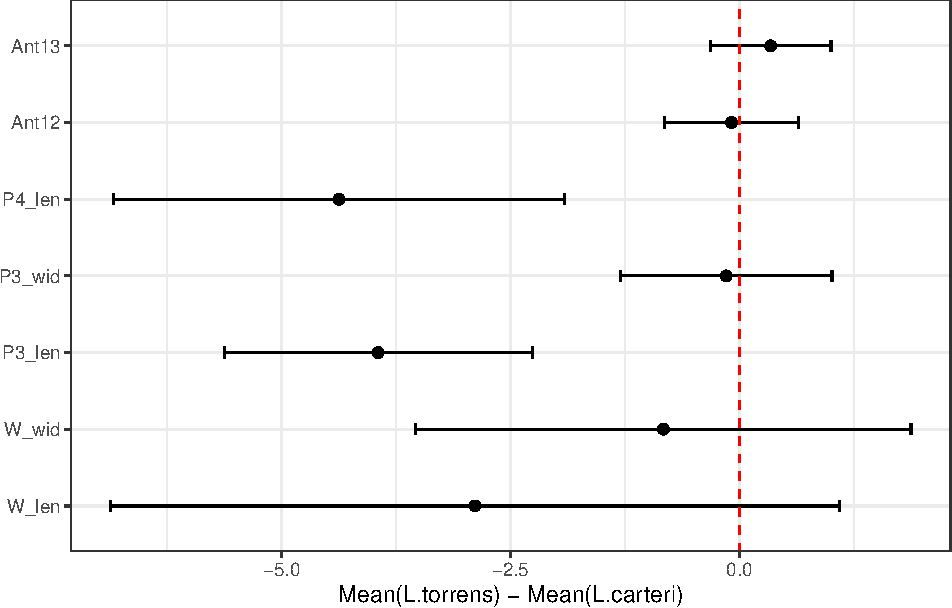
\includegraphics[width=0.85\linewidth]{Midterm_Report_files/figure-latex/ci-plot-1} 

}

\caption{Bonferroni 95\% simultaneous CIs for mean differences (raw scale).}\label{fig:ci-plot}
\end{figure}

\section{Discussion and conclusion}\label{discussion-and-conclusion}

The univariate diagnostics highlighted heterogeneous skewness across the
seven morphometric variables, with Box-Cox parameters ranging from
\(\lambda \approx 0\) (third-palp variables) to \(\lambda \approx 2\)
(wing dimensions). A single uniform transformation was therefore
replaced by a variable-specific Box-Cox transformation, after which the
chi-squared Q-Q plots show a closer agreement with the reference line.
Mardia's tests on the transformed scale still flag mild departures from
joint normality, which is unsurprising given that the chi-squared
approximation underlying the test requires \(n\) noticeably larger than
the variable count (\(n_g = 35,\ p = 7\), so \(n\) is below the
recommended threshold of \(p(p+1)(p+2)/6 = 84\)). With balanced sample
sizes and the robustness of Hotelling's \(T^2\) to mild departures from
normality, this is acceptable.

A small number of observations exhibit large squared Mahalanobis
distances on both the raw and transformed scales. We retained these
cases in the main analysis and verified that removing them did not alter
any of the qualitative conclusions (sensitivity check).

Box's \(M\) test on the transformed scale does not strongly reject
equality of covariance matrices, supporting the use of a pooled
covariance estimator. Hotelling's \(T^2\) is highly significant on both
the raw and Box-Cox scales (Section 7), confirming that the mean
morphometric profiles of \emph{L. torrens} and \emph{L. carteri} differ.

Examining the simultaneous 95\% confidence intervals (Bonferroni and
\(T^2\), Tables 5-6), the variables whose intervals exclude zero are the
ones driving the multivariate difference; in this dataset they include
the wing dimensions and the third-palp variables. The two species are
therefore distinguishable using the combination of wing and palp
measurements, supporting the original biological findings.

Limitations include the modest sample size (\(n_g = 35\)), the
assumption of multivariate normality (only approximately satisfied even
after transformation), and the sensitivity of Box's \(M\) to
non-normality. Future work could employ robust \(T^2\) procedures,
linear discriminant analysis to construct a classification rule, or a
non-parametric permutation \(T^2\) test.

\section{Appendix A: All R code}\label{appendix-a-all-r-code}

\begin{Shaded}
\begin{Highlighting}[]
\NormalTok{knitr}\SpecialCharTok{::}\NormalTok{opts\_chunk}\SpecialCharTok{$}\FunctionTok{set}\NormalTok{(}
  \AttributeTok{echo       =} \ConstantTok{FALSE}\NormalTok{,    }\CommentTok{\# hide code in the body; reprinted in appendix}
  \AttributeTok{message    =} \ConstantTok{FALSE}\NormalTok{,}
  \AttributeTok{warning    =} \ConstantTok{FALSE}\NormalTok{,}
  \AttributeTok{fig.align  =} \StringTok{"center"}\NormalTok{,}
  \AttributeTok{fig.width  =} \FloatTok{6.5}\NormalTok{,}
  \AttributeTok{fig.height =} \FloatTok{4.2}\NormalTok{,}
  \AttributeTok{out.width  =} \StringTok{"85\%"}
\NormalTok{)}

\CommentTok{\# {-}{-}{-}{-} Required packages {-}{-}{-}{-}{-}{-}{-}{-}{-}{-}{-}{-}{-}{-}{-}{-}{-}{-}{-}{-}{-}{-}{-}{-}{-}{-}{-}{-}{-}{-}{-}{-}{-}{-}{-}{-}{-}{-}{-}{-}{-}{-}{-}{-}{-}{-}{-}{-}{-}{-}{-}{-}{-}}
\NormalTok{pkgs }\OtherTok{\textless{}{-}} \FunctionTok{c}\NormalTok{(}\StringTok{"readxl"}\NormalTok{, }\StringTok{"dplyr"}\NormalTok{, }\StringTok{"tidyr"}\NormalTok{, }\StringTok{"ggplot2"}\NormalTok{, }\StringTok{"GGally"}\NormalTok{,}
          \StringTok{"MVN"}\NormalTok{, }\StringTok{"biotools"}\NormalTok{, }\StringTok{"ICSNP"}\NormalTok{, }\StringTok{"MASS"}\NormalTok{, }\StringTok{"knitr"}\NormalTok{, }\StringTok{"kableExtra"}\NormalTok{)}
\NormalTok{new  }\OtherTok{\textless{}{-}}\NormalTok{ pkgs[}\SpecialCharTok{!}\NormalTok{pkgs }\SpecialCharTok{\%in\%} \FunctionTok{installed.packages}\NormalTok{()[, }\StringTok{"Package"}\NormalTok{]]}
\ControlFlowTok{if}\NormalTok{ (}\FunctionTok{length}\NormalTok{(new)) }\FunctionTok{install.packages}\NormalTok{(new, }\AttributeTok{repos =} \StringTok{"https://cloud.r{-}project.org"}\NormalTok{)}
\FunctionTok{invisible}\NormalTok{(}\FunctionTok{lapply}\NormalTok{(pkgs, library, }\AttributeTok{character.only =} \ConstantTok{TRUE}\NormalTok{))}

\FunctionTok{set.seed}\NormalTok{(}\DecValTok{2025}\NormalTok{)}
\NormalTok{df }\OtherTok{\textless{}{-}} \FunctionTok{read\_excel}\NormalTok{(}\StringTok{"flies.xls"}\NormalTok{)}
\FunctionTok{names}\NormalTok{(df) }\OtherTok{\textless{}{-}} \FunctionTok{c}\NormalTok{(}\StringTok{"W\_len"}\NormalTok{, }\StringTok{"W\_wid"}\NormalTok{, }\StringTok{"P3\_len"}\NormalTok{, }\StringTok{"P3\_wid"}\NormalTok{,}
               \StringTok{"P4\_len"}\NormalTok{, }\StringTok{"Ant12"}\NormalTok{, }\StringTok{"Ant13"}\NormalTok{, }\StringTok{"Species"}\NormalTok{)}
\NormalTok{df }\OtherTok{\textless{}{-}}\NormalTok{ df }\SpecialCharTok{\%\textgreater{}\%}
  \FunctionTok{mutate}\NormalTok{(}\AttributeTok{Species =} \FunctionTok{factor}\NormalTok{(Species, }\AttributeTok{levels =} \FunctionTok{c}\NormalTok{(}\DecValTok{0}\NormalTok{, }\DecValTok{1}\NormalTok{),}
                          \AttributeTok{labels =} \FunctionTok{c}\NormalTok{(}\StringTok{"L.torrens"}\NormalTok{, }\StringTok{"L.carteri"}\NormalTok{)))}
\FunctionTok{glimpse}\NormalTok{(df)}
\NormalTok{X  }\OtherTok{\textless{}{-}} \FunctionTok{as.matrix}\NormalTok{(df[, }\DecValTok{1}\SpecialCharTok{:}\DecValTok{7}\NormalTok{])}
\NormalTok{g  }\OtherTok{\textless{}{-}}\NormalTok{ df}\SpecialCharTok{$}\NormalTok{Species}
\NormalTok{X1 }\OtherTok{\textless{}{-}}\NormalTok{ X[g }\SpecialCharTok{==} \StringTok{"L.torrens"}\NormalTok{, ]   }\CommentTok{\# n1 = 35}
\NormalTok{X2 }\OtherTok{\textless{}{-}}\NormalTok{ X[g }\SpecialCharTok{==} \StringTok{"L.carteri"}\NormalTok{, ]   }\CommentTok{\# n2 = 35}
\NormalTok{n1 }\OtherTok{\textless{}{-}} \FunctionTok{nrow}\NormalTok{(X1); n2 }\OtherTok{\textless{}{-}} \FunctionTok{nrow}\NormalTok{(X2); p }\OtherTok{\textless{}{-}} \FunctionTok{ncol}\NormalTok{(X)}
\NormalTok{desc }\OtherTok{\textless{}{-}}\NormalTok{ df }\SpecialCharTok{\%\textgreater{}\%}
  \FunctionTok{pivot\_longer}\NormalTok{(}\SpecialCharTok{{-}}\NormalTok{Species, }\AttributeTok{names\_to =} \StringTok{"Variable"}\NormalTok{, }\AttributeTok{values\_to =} \StringTok{"Value"}\NormalTok{) }\SpecialCharTok{\%\textgreater{}\%}
  \FunctionTok{group\_by}\NormalTok{(Variable, Species) }\SpecialCharTok{\%\textgreater{}\%}
  \FunctionTok{summarise}\NormalTok{(}\AttributeTok{Mean =} \FunctionTok{mean}\NormalTok{(Value), }\AttributeTok{SD =} \FunctionTok{sd}\NormalTok{(Value), }\AttributeTok{.groups =} \StringTok{"drop"}\NormalTok{) }\SpecialCharTok{\%\textgreater{}\%}
  \FunctionTok{pivot\_wider}\NormalTok{(}\AttributeTok{names\_from =}\NormalTok{ Species, }\AttributeTok{values\_from =} \FunctionTok{c}\NormalTok{(Mean, SD)) }\SpecialCharTok{\%\textgreater{}\%}
  \FunctionTok{mutate}\NormalTok{(}\AttributeTok{Diff =}\NormalTok{ Mean\_L.torrens }\SpecialCharTok{{-}}\NormalTok{ Mean\_L.carteri)}

\FunctionTok{kable}\NormalTok{(desc, }\AttributeTok{digits =} \DecValTok{2}\NormalTok{, }\AttributeTok{booktabs =} \ConstantTok{TRUE}\NormalTok{,}
      \AttributeTok{caption =} \StringTok{"Per{-}species means and standard deviations."}\NormalTok{) }\SpecialCharTok{\%\textgreater{}\%}
  \FunctionTok{kable\_styling}\NormalTok{(}\AttributeTok{latex\_options =} \StringTok{"hold\_position"}\NormalTok{)}
\NormalTok{df }\SpecialCharTok{\%\textgreater{}\%}
  \FunctionTok{pivot\_longer}\NormalTok{(}\SpecialCharTok{{-}}\NormalTok{Species, }\AttributeTok{names\_to =} \StringTok{"Variable"}\NormalTok{, }\AttributeTok{values\_to =} \StringTok{"Value"}\NormalTok{) }\SpecialCharTok{\%\textgreater{}\%}
  \FunctionTok{ggplot}\NormalTok{(}\FunctionTok{aes}\NormalTok{(Species, Value, }\AttributeTok{fill =}\NormalTok{ Species)) }\SpecialCharTok{+}
  \FunctionTok{geom\_boxplot}\NormalTok{(}\AttributeTok{alpha =} \FloatTok{0.7}\NormalTok{) }\SpecialCharTok{+}
  \FunctionTok{facet\_wrap}\NormalTok{(}\SpecialCharTok{\textasciitilde{}}\NormalTok{ Variable, }\AttributeTok{scales =} \StringTok{"free\_y"}\NormalTok{, }\AttributeTok{ncol =} \DecValTok{4}\NormalTok{) }\SpecialCharTok{+}
  \FunctionTok{theme\_bw}\NormalTok{() }\SpecialCharTok{+} \FunctionTok{theme}\NormalTok{(}\AttributeTok{legend.position =} \StringTok{"none"}\NormalTok{)}
\FunctionTok{ggpairs}\NormalTok{(df, }\AttributeTok{columns =} \DecValTok{1}\SpecialCharTok{:}\DecValTok{7}\NormalTok{, }\FunctionTok{aes}\NormalTok{(}\AttributeTok{colour =}\NormalTok{ Species, }\AttributeTok{alpha =} \FloatTok{0.6}\NormalTok{),}
        \AttributeTok{upper =} \FunctionTok{list}\NormalTok{(}\AttributeTok{continuous =} \FunctionTok{wrap}\NormalTok{(}\StringTok{"cor"}\NormalTok{, }\AttributeTok{size =} \FloatTok{2.6}\NormalTok{))) }\SpecialCharTok{+}
  \FunctionTok{theme\_bw}\NormalTok{(}\AttributeTok{base\_size =} \DecValTok{8}\NormalTok{)}
\NormalTok{op }\OtherTok{\textless{}{-}} \FunctionTok{par}\NormalTok{(}\AttributeTok{mfrow =} \FunctionTok{c}\NormalTok{(}\DecValTok{7}\NormalTok{, }\DecValTok{2}\NormalTok{), }\AttributeTok{mar =} \FunctionTok{c}\NormalTok{(}\DecValTok{3}\NormalTok{, }\DecValTok{3}\NormalTok{, }\DecValTok{2}\NormalTok{, }\DecValTok{1}\NormalTok{), }\AttributeTok{mgp =} \FunctionTok{c}\NormalTok{(}\FloatTok{1.6}\NormalTok{, }\FloatTok{0.5}\NormalTok{, }\DecValTok{0}\NormalTok{))}
\ControlFlowTok{for}\NormalTok{ (k }\ControlFlowTok{in} \DecValTok{1}\SpecialCharTok{:}\NormalTok{p) \{}
  \FunctionTok{qqnorm}\NormalTok{(X1[, k], }\AttributeTok{main =} \FunctionTok{paste}\NormalTok{(}\FunctionTok{colnames}\NormalTok{(X)[k], }\StringTok{"  L.torrens"}\NormalTok{))}
  \FunctionTok{qqline}\NormalTok{(X1[, k], }\AttributeTok{col =} \StringTok{"red"}\NormalTok{)}
  \FunctionTok{qqnorm}\NormalTok{(X2[, k], }\AttributeTok{main =} \FunctionTok{paste}\NormalTok{(}\FunctionTok{colnames}\NormalTok{(X)[k], }\StringTok{"  L.carteri"}\NormalTok{))}
  \FunctionTok{qqline}\NormalTok{(X2[, k], }\AttributeTok{col =} \StringTok{"red"}\NormalTok{)}
\NormalTok{\}}
\FunctionTok{par}\NormalTok{(op)}
\NormalTok{shap }\OtherTok{\textless{}{-}} \FunctionTok{sapply}\NormalTok{(}\DecValTok{1}\SpecialCharTok{:}\NormalTok{p, }\ControlFlowTok{function}\NormalTok{(k) \{}
  \FunctionTok{c}\NormalTok{(}\AttributeTok{L.torrens =} \FunctionTok{shapiro.test}\NormalTok{(X1[, k])}\SpecialCharTok{$}\NormalTok{p.value,}
    \AttributeTok{L.carteri =} \FunctionTok{shapiro.test}\NormalTok{(X2[, k])}\SpecialCharTok{$}\NormalTok{p.value)}
\NormalTok{\})}
\FunctionTok{colnames}\NormalTok{(shap) }\OtherTok{\textless{}{-}} \FunctionTok{colnames}\NormalTok{(X)}
\FunctionTok{kable}\NormalTok{(}\FunctionTok{t}\NormalTok{(}\FunctionTok{round}\NormalTok{(shap, }\DecValTok{3}\NormalTok{)), }\AttributeTok{booktabs =} \ConstantTok{TRUE}\NormalTok{,}
      \AttributeTok{caption =} \StringTok{"Shapiro–Wilk p{-}values (variables in rows)."}\NormalTok{) }\SpecialCharTok{\%\textgreater{}\%}
  \FunctionTok{kable\_styling}\NormalTok{(}\AttributeTok{latex\_options =} \StringTok{"hold\_position"}\NormalTok{)}
\CommentTok{\# Self{-}contained Mardia test: avoids MVN 6.x output formatting that}
\CommentTok{\# breaks LaTeX (Unicode glyphs, special chars).}
\NormalTok{mardia\_test }\OtherTok{\textless{}{-}} \ControlFlowTok{function}\NormalTok{(X) \{}
\NormalTok{  X }\OtherTok{\textless{}{-}} \FunctionTok{as.matrix}\NormalTok{(X); n }\OtherTok{\textless{}{-}} \FunctionTok{nrow}\NormalTok{(X); p }\OtherTok{\textless{}{-}} \FunctionTok{ncol}\NormalTok{(X)}
\NormalTok{  Xc }\OtherTok{\textless{}{-}} \FunctionTok{scale}\NormalTok{(X, }\AttributeTok{center =} \ConstantTok{TRUE}\NormalTok{, }\AttributeTok{scale =} \ConstantTok{FALSE}\NormalTok{)}
\NormalTok{  S  }\OtherTok{\textless{}{-}} \FunctionTok{cov}\NormalTok{(X) }\SpecialCharTok{*}\NormalTok{ (n }\SpecialCharTok{{-}} \DecValTok{1}\NormalTok{) }\SpecialCharTok{/}\NormalTok{ n}
\NormalTok{  D  }\OtherTok{\textless{}{-}}\NormalTok{ Xc }\SpecialCharTok{\%*\%} \FunctionTok{solve}\NormalTok{(S) }\SpecialCharTok{\%*\%} \FunctionTok{t}\NormalTok{(Xc)}

\NormalTok{  b1p }\OtherTok{\textless{}{-}} \FunctionTok{sum}\NormalTok{(D}\SpecialCharTok{\^{}}\DecValTok{3}\NormalTok{) }\SpecialCharTok{/}\NormalTok{ n}\SpecialCharTok{\^{}}\DecValTok{2}
\NormalTok{  b2p }\OtherTok{\textless{}{-}} \FunctionTok{sum}\NormalTok{(}\FunctionTok{diag}\NormalTok{(D)}\SpecialCharTok{\^{}}\DecValTok{2}\NormalTok{) }\SpecialCharTok{/}\NormalTok{ n}
\NormalTok{  k1  }\OtherTok{\textless{}{-}}\NormalTok{ n }\SpecialCharTok{*}\NormalTok{ b1p }\SpecialCharTok{/} \DecValTok{6}
\NormalTok{  df1 }\OtherTok{\textless{}{-}}\NormalTok{ p }\SpecialCharTok{*}\NormalTok{ (p }\SpecialCharTok{+} \DecValTok{1}\NormalTok{) }\SpecialCharTok{*}\NormalTok{ (p }\SpecialCharTok{+} \DecValTok{2}\NormalTok{) }\SpecialCharTok{/} \DecValTok{6}
\NormalTok{  p1  }\OtherTok{\textless{}{-}} \FunctionTok{pchisq}\NormalTok{(k1, df1, }\AttributeTok{lower.tail =} \ConstantTok{FALSE}\NormalTok{)}
\NormalTok{  z2  }\OtherTok{\textless{}{-}}\NormalTok{ (b2p }\SpecialCharTok{{-}}\NormalTok{ p }\SpecialCharTok{*}\NormalTok{ (p }\SpecialCharTok{+} \DecValTok{2}\NormalTok{)) }\SpecialCharTok{/} \FunctionTok{sqrt}\NormalTok{(}\DecValTok{8} \SpecialCharTok{*}\NormalTok{ p }\SpecialCharTok{*}\NormalTok{ (p }\SpecialCharTok{+} \DecValTok{2}\NormalTok{) }\SpecialCharTok{/}\NormalTok{ n)}
\NormalTok{  p2  }\OtherTok{\textless{}{-}} \DecValTok{2} \SpecialCharTok{*} \FunctionTok{pnorm}\NormalTok{(}\SpecialCharTok{{-}}\FunctionTok{abs}\NormalTok{(z2))}

  \FunctionTok{data.frame}\NormalTok{(}
    \AttributeTok{Test       =} \FunctionTok{c}\NormalTok{(}\StringTok{"Mardia skewness"}\NormalTok{, }\StringTok{"Mardia kurtosis"}\NormalTok{),}
    \AttributeTok{Statistic  =} \FunctionTok{round}\NormalTok{(}\FunctionTok{c}\NormalTok{(k1, z2), }\DecValTok{3}\NormalTok{),}
    \AttributeTok{df         =} \FunctionTok{c}\NormalTok{(df1, }\ConstantTok{NA}\NormalTok{),}
    \AttributeTok{p\_value    =} \FunctionTok{signif}\NormalTok{(}\FunctionTok{c}\NormalTok{(p1, p2), }\DecValTok{3}\NormalTok{),}
    \AttributeTok{Reject\_H0  =} \FunctionTok{ifelse}\NormalTok{(}\FunctionTok{c}\NormalTok{(p1, p2) }\SpecialCharTok{\textless{}} \FloatTok{0.05}\NormalTok{, }\StringTok{"Yes"}\NormalTok{, }\StringTok{"No"}\NormalTok{),}
    \AttributeTok{stringsAsFactors =} \ConstantTok{FALSE}
\NormalTok{  )}
\NormalTok{\}}

\FunctionTok{kable}\NormalTok{(}\FunctionTok{mardia\_test}\NormalTok{(X1), }\AttributeTok{booktabs =} \ConstantTok{TRUE}\NormalTok{,}
      \AttributeTok{caption =} \StringTok{"Mardia test of multivariate normality, L. torrens."}\NormalTok{) }\SpecialCharTok{\%\textgreater{}\%}
  \FunctionTok{kable\_styling}\NormalTok{(}\AttributeTok{latex\_options =} \StringTok{"hold\_position"}\NormalTok{)}
\FunctionTok{kable}\NormalTok{(}\FunctionTok{mardia\_test}\NormalTok{(X2), }\AttributeTok{booktabs =} \ConstantTok{TRUE}\NormalTok{,}
      \AttributeTok{caption =} \StringTok{"Mardia test of multivariate normality, L. carteri."}\NormalTok{) }\SpecialCharTok{\%\textgreater{}\%}
  \FunctionTok{kable\_styling}\NormalTok{(}\AttributeTok{latex\_options =} \StringTok{"hold\_position"}\NormalTok{)}
\NormalTok{chiQQ }\OtherTok{\textless{}{-}} \ControlFlowTok{function}\NormalTok{(M, ttl) \{}
\NormalTok{  d2   }\OtherTok{\textless{}{-}} \FunctionTok{mahalanobis}\NormalTok{(M, }\FunctionTok{colMeans}\NormalTok{(M), }\FunctionTok{cov}\NormalTok{(M))}
\NormalTok{  qchi }\OtherTok{\textless{}{-}} \FunctionTok{qchisq}\NormalTok{(}\FunctionTok{ppoints}\NormalTok{(}\FunctionTok{nrow}\NormalTok{(M)), }\AttributeTok{df =} \FunctionTok{ncol}\NormalTok{(M))}
  \FunctionTok{plot}\NormalTok{(qchi, }\FunctionTok{sort}\NormalTok{(d2), }\AttributeTok{pch =} \DecValTok{20}\NormalTok{, }\AttributeTok{main =}\NormalTok{ ttl,}
       \AttributeTok{xlab =} \FunctionTok{expression}\NormalTok{(chi[}\DecValTok{7}\NormalTok{]}\SpecialCharTok{\^{}}\DecValTok{2} \SpecialCharTok{\textasciitilde{}} \StringTok{"quantile"}\NormalTok{),}
       \AttributeTok{ylab =} \StringTok{"ordered  d\^{}2"}\NormalTok{)}
  \FunctionTok{abline}\NormalTok{(}\DecValTok{0}\NormalTok{, }\DecValTok{1}\NormalTok{, }\AttributeTok{col =} \StringTok{"red"}\NormalTok{, }\AttributeTok{lwd =} \FloatTok{1.5}\NormalTok{)}
\NormalTok{\}}
\NormalTok{op }\OtherTok{\textless{}{-}} \FunctionTok{par}\NormalTok{(}\AttributeTok{mfrow =} \FunctionTok{c}\NormalTok{(}\DecValTok{1}\NormalTok{, }\DecValTok{2}\NormalTok{))}
\FunctionTok{chiQQ}\NormalTok{(X1, }\StringTok{"L. torrens"}\NormalTok{); }\FunctionTok{chiQQ}\NormalTok{(X2, }\StringTok{"L. carteri"}\NormalTok{); }\FunctionTok{par}\NormalTok{(op)}
\NormalTok{cutoff }\OtherTok{\textless{}{-}} \FunctionTok{qchisq}\NormalTok{(}\FloatTok{0.975}\NormalTok{, }\AttributeTok{df =}\NormalTok{ p)        }\CommentTok{\# \textasciitilde{} 16.01}
\NormalTok{d2\_1   }\OtherTok{\textless{}{-}} \FunctionTok{mahalanobis}\NormalTok{(X1, }\FunctionTok{colMeans}\NormalTok{(X1), }\FunctionTok{cov}\NormalTok{(X1))}
\NormalTok{d2\_2   }\OtherTok{\textless{}{-}} \FunctionTok{mahalanobis}\NormalTok{(X2, }\FunctionTok{colMeans}\NormalTok{(X2), }\FunctionTok{cov}\NormalTok{(X2))}

\NormalTok{out\_tbl }\OtherTok{\textless{}{-}} \FunctionTok{data.frame}\NormalTok{(}
  \AttributeTok{Species  =} \FunctionTok{c}\NormalTok{(}\FunctionTok{rep}\NormalTok{(}\StringTok{"L.torrens"}\NormalTok{, n1), }\FunctionTok{rep}\NormalTok{(}\StringTok{"L.carteri"}\NormalTok{, n2)),}
  \AttributeTok{Index    =} \FunctionTok{c}\NormalTok{(}\FunctionTok{seq\_len}\NormalTok{(n1), }\FunctionTok{seq\_len}\NormalTok{(n2)),}
  \AttributeTok{D2       =} \FunctionTok{c}\NormalTok{(d2\_1, d2\_2),}
  \AttributeTok{Outlier  =} \FunctionTok{c}\NormalTok{(d2\_1, d2\_2) }\SpecialCharTok{\textgreater{}}\NormalTok{ cutoff}
\NormalTok{)}
\FunctionTok{kable}\NormalTok{(}\FunctionTok{subset}\NormalTok{(out\_tbl, Outlier),}
      \AttributeTok{digits =} \DecValTok{2}\NormalTok{, }\AttributeTok{booktabs =} \ConstantTok{TRUE}\NormalTok{,}
      \AttributeTok{caption =} \FunctionTok{sprintf}\NormalTok{(}\StringTok{"Cases with $d\^{}2 \textgreater{} \%.2f$."}\NormalTok{, cutoff)) }\SpecialCharTok{\%\textgreater{}\%}
  \FunctionTok{kable\_styling}\NormalTok{(}\AttributeTok{latex\_options =} \StringTok{"hold\_position"}\NormalTok{)}
\NormalTok{lambda }\OtherTok{\textless{}{-}} \FunctionTok{sapply}\NormalTok{(}\DecValTok{1}\SpecialCharTok{:}\NormalTok{p, }\ControlFlowTok{function}\NormalTok{(k) \{}
\NormalTok{  bc }\OtherTok{\textless{}{-}}\NormalTok{ MASS}\SpecialCharTok{::}\FunctionTok{boxcox}\NormalTok{(X[, k] }\SpecialCharTok{\textasciitilde{}} \DecValTok{1}\NormalTok{, }\AttributeTok{plotit =} \ConstantTok{FALSE}\NormalTok{)}
\NormalTok{  bc}\SpecialCharTok{$}\NormalTok{x[}\FunctionTok{which.max}\NormalTok{(bc}\SpecialCharTok{$}\NormalTok{y)]}
\NormalTok{\})}
\FunctionTok{names}\NormalTok{(lambda) }\OtherTok{\textless{}{-}} \FunctionTok{colnames}\NormalTok{(X)}
\FunctionTok{kable}\NormalTok{(}\FunctionTok{t}\NormalTok{(}\FunctionTok{round}\NormalTok{(lambda, }\DecValTok{2}\NormalTok{)), }\AttributeTok{booktabs =} \ConstantTok{TRUE}\NormalTok{,}
      \AttributeTok{caption =} \StringTok{"Optimal Box{-}Cox lambdas (per variable)."}\NormalTok{) }\SpecialCharTok{\%\textgreater{}\%}
  \FunctionTok{kable\_styling}\NormalTok{(}\AttributeTok{latex\_options =} \StringTok{"hold\_position"}\NormalTok{)}
\CommentTok{\# Box{-}Cox helper: log when lambda is (numerically) zero.}
\NormalTok{bc\_apply }\OtherTok{\textless{}{-}} \ControlFlowTok{function}\NormalTok{(x, lam) \{}
  \ControlFlowTok{if}\NormalTok{ (}\FunctionTok{abs}\NormalTok{(lam) }\SpecialCharTok{\textless{}} \FloatTok{1e{-}6}\NormalTok{) }\FunctionTok{log}\NormalTok{(x) }\ControlFlowTok{else}\NormalTok{ (x}\SpecialCharTok{\^{}}\NormalTok{lam }\SpecialCharTok{{-}} \DecValTok{1}\NormalTok{) }\SpecialCharTok{/}\NormalTok{ lam}
\NormalTok{\}}

\NormalTok{Xbc  }\OtherTok{\textless{}{-}} \FunctionTok{sapply}\NormalTok{(}\DecValTok{1}\SpecialCharTok{:}\NormalTok{p, }\ControlFlowTok{function}\NormalTok{(k) }\FunctionTok{bc\_apply}\NormalTok{(X[, k], lambda[k]))}
\FunctionTok{colnames}\NormalTok{(Xbc) }\OtherTok{\textless{}{-}} \FunctionTok{colnames}\NormalTok{(X)}
\NormalTok{X1bc }\OtherTok{\textless{}{-}}\NormalTok{ Xbc[g }\SpecialCharTok{==} \StringTok{"L.torrens"}\NormalTok{, ]}
\NormalTok{X2bc }\OtherTok{\textless{}{-}}\NormalTok{ Xbc[g }\SpecialCharTok{==} \StringTok{"L.carteri"}\NormalTok{, ]}

\FunctionTok{kable}\NormalTok{(}\FunctionTok{mardia\_test}\NormalTok{(X1bc), }\AttributeTok{booktabs =} \ConstantTok{TRUE}\NormalTok{,}
      \AttributeTok{caption =} \StringTok{"Mardia test after variable{-}specific Box{-}Cox, L. torrens."}\NormalTok{) }\SpecialCharTok{\%\textgreater{}\%}
  \FunctionTok{kable\_styling}\NormalTok{(}\AttributeTok{latex\_options =} \StringTok{"hold\_position"}\NormalTok{)}
\FunctionTok{kable}\NormalTok{(}\FunctionTok{mardia\_test}\NormalTok{(X2bc), }\AttributeTok{booktabs =} \ConstantTok{TRUE}\NormalTok{,}
      \AttributeTok{caption =} \StringTok{"Mardia test after variable{-}specific Box{-}Cox, L. carteri."}\NormalTok{) }\SpecialCharTok{\%\textgreater{}\%}
  \FunctionTok{kable\_styling}\NormalTok{(}\AttributeTok{latex\_options =} \StringTok{"hold\_position"}\NormalTok{)}
\NormalTok{op }\OtherTok{\textless{}{-}} \FunctionTok{par}\NormalTok{(}\AttributeTok{mfrow =} \FunctionTok{c}\NormalTok{(}\DecValTok{1}\NormalTok{, }\DecValTok{2}\NormalTok{))}
\FunctionTok{chiQQ}\NormalTok{(X1bc, }\StringTok{"Box{-}Cox  L. torrens"}\NormalTok{)}
\FunctionTok{chiQQ}\NormalTok{(X2bc, }\StringTok{"Box{-}Cox  L. carteri"}\NormalTok{)}
\FunctionTok{par}\NormalTok{(op)}
\CommentTok{\# Re{-}check Mahalanobis outliers on the transformed scale}
\NormalTok{d2\_1bc }\OtherTok{\textless{}{-}} \FunctionTok{mahalanobis}\NormalTok{(X1bc, }\FunctionTok{colMeans}\NormalTok{(X1bc), }\FunctionTok{cov}\NormalTok{(X1bc))}
\NormalTok{d2\_2bc }\OtherTok{\textless{}{-}} \FunctionTok{mahalanobis}\NormalTok{(X2bc, }\FunctionTok{colMeans}\NormalTok{(X2bc), }\FunctionTok{cov}\NormalTok{(X2bc))}
\NormalTok{out\_bc }\OtherTok{\textless{}{-}} \FunctionTok{data.frame}\NormalTok{(}
  \AttributeTok{Species =} \FunctionTok{c}\NormalTok{(}\FunctionTok{rep}\NormalTok{(}\StringTok{"L.torrens"}\NormalTok{, n1), }\FunctionTok{rep}\NormalTok{(}\StringTok{"L.carteri"}\NormalTok{, n2)),}
  \AttributeTok{Index   =} \FunctionTok{c}\NormalTok{(}\FunctionTok{seq\_len}\NormalTok{(n1), }\FunctionTok{seq\_len}\NormalTok{(n2)),}
  \AttributeTok{D2      =} \FunctionTok{c}\NormalTok{(d2\_1bc, d2\_2bc),}
  \AttributeTok{Outlier =} \FunctionTok{c}\NormalTok{(d2\_1bc, d2\_2bc) }\SpecialCharTok{\textgreater{}}\NormalTok{ cutoff}
\NormalTok{)}
\FunctionTok{kable}\NormalTok{(}\FunctionTok{subset}\NormalTok{(out\_bc, Outlier), }\AttributeTok{digits =} \DecValTok{2}\NormalTok{, }\AttributeTok{booktabs =} \ConstantTok{TRUE}\NormalTok{,}
      \AttributeTok{caption =} \FunctionTok{sprintf}\NormalTok{(}
        \StringTok{"Cases with $d\^{}2 \textgreater{} \%.2f$ after Box{-}Cox transformation."}\NormalTok{, cutoff)) }\SpecialCharTok{\%\textgreater{}\%}
  \FunctionTok{kable\_styling}\NormalTok{(}\AttributeTok{latex\_options =} \StringTok{"hold\_position"}\NormalTok{)}
\CommentTok{\# Indices of multivariate outliers on the raw scale}
\NormalTok{out1\_raw }\OtherTok{\textless{}{-}} \FunctionTok{which}\NormalTok{(d2\_1 }\SpecialCharTok{\textgreater{}}\NormalTok{ cutoff)}
\NormalTok{out2\_raw }\OtherTok{\textless{}{-}} \FunctionTok{which}\NormalTok{(d2\_2 }\SpecialCharTok{\textgreater{}}\NormalTok{ cutoff)}

\NormalTok{X1c }\OtherTok{\textless{}{-}}\NormalTok{ X1[}\FunctionTok{setdiff}\NormalTok{(}\FunctionTok{seq\_len}\NormalTok{(n1), out1\_raw), , drop }\OtherTok{=} \ConstantTok{FALSE}\NormalTok{]}
\NormalTok{X2c }\OtherTok{\textless{}{-}}\NormalTok{ X2[}\FunctionTok{setdiff}\NormalTok{(}\FunctionTok{seq\_len}\NormalTok{(n2), out2\_raw), , drop }\OtherTok{=} \ConstantTok{FALSE}\NormalTok{]}
\NormalTok{Xc  }\OtherTok{\textless{}{-}} \FunctionTok{rbind}\NormalTok{(X1c, X2c)}
\NormalTok{gc  }\OtherTok{\textless{}{-}} \FunctionTok{factor}\NormalTok{(}\FunctionTok{c}\NormalTok{(}\FunctionTok{rep}\NormalTok{(}\StringTok{"L.torrens"}\NormalTok{, }\FunctionTok{nrow}\NormalTok{(X1c)),}
                \FunctionTok{rep}\NormalTok{(}\StringTok{"L.carteri"}\NormalTok{, }\FunctionTok{nrow}\NormalTok{(X2c))),}
              \AttributeTok{levels =} \FunctionTok{c}\NormalTok{(}\StringTok{"L.torrens"}\NormalTok{, }\StringTok{"L.carteri"}\NormalTok{))}

\CommentTok{\# Re{-}estimate Box{-}Cox lambdas on the cleaned data}
\NormalTok{lambda\_c }\OtherTok{\textless{}{-}} \FunctionTok{sapply}\NormalTok{(}\DecValTok{1}\SpecialCharTok{:}\NormalTok{p, }\ControlFlowTok{function}\NormalTok{(k) \{}
\NormalTok{  bc }\OtherTok{\textless{}{-}}\NormalTok{ MASS}\SpecialCharTok{::}\FunctionTok{boxcox}\NormalTok{(Xc[, k] }\SpecialCharTok{\textasciitilde{}} \DecValTok{1}\NormalTok{, }\AttributeTok{plotit =} \ConstantTok{FALSE}\NormalTok{)}
\NormalTok{  bc}\SpecialCharTok{$}\NormalTok{x[}\FunctionTok{which.max}\NormalTok{(bc}\SpecialCharTok{$}\NormalTok{y)]}
\NormalTok{\})}
\FunctionTok{names}\NormalTok{(lambda\_c) }\OtherTok{\textless{}{-}} \FunctionTok{colnames}\NormalTok{(X)}

\NormalTok{Xbc\_c  }\OtherTok{\textless{}{-}} \FunctionTok{sapply}\NormalTok{(}\DecValTok{1}\SpecialCharTok{:}\NormalTok{p, }\ControlFlowTok{function}\NormalTok{(k) }\FunctionTok{bc\_apply}\NormalTok{(Xc[, k], lambda\_c[k]))}
\FunctionTok{colnames}\NormalTok{(Xbc\_c) }\OtherTok{\textless{}{-}} \FunctionTok{colnames}\NormalTok{(X)}
\NormalTok{X1bc\_c }\OtherTok{\textless{}{-}}\NormalTok{ Xbc\_c[gc }\SpecialCharTok{==} \StringTok{"L.torrens"}\NormalTok{, ]}
\NormalTok{X2bc\_c }\OtherTok{\textless{}{-}}\NormalTok{ Xbc\_c[gc }\SpecialCharTok{==} \StringTok{"L.carteri"}\NormalTok{, ]}
\FunctionTok{kable}\NormalTok{(}\FunctionTok{rbind}\NormalTok{(}\StringTok{\textasciigrave{}}\AttributeTok{Full sample}\StringTok{\textasciigrave{}}     \OtherTok{=} \FunctionTok{round}\NormalTok{(lambda,   }\DecValTok{2}\NormalTok{),}
            \StringTok{\textasciigrave{}}\AttributeTok{Outliers removed}\StringTok{\textasciigrave{}}\OtherTok{=} \FunctionTok{round}\NormalTok{(lambda\_c, }\DecValTok{2}\NormalTok{)),}
      \AttributeTok{booktabs =} \ConstantTok{TRUE}\NormalTok{,}
      \AttributeTok{caption =} \StringTok{"Optimal Box{-}Cox lambdas, before vs. after outlier removal."}\NormalTok{) }\SpecialCharTok{\%\textgreater{}\%}
  \FunctionTok{kable\_styling}\NormalTok{(}\AttributeTok{latex\_options =} \StringTok{"hold\_position"}\NormalTok{)}
\FunctionTok{kable}\NormalTok{(}\FunctionTok{mardia\_test}\NormalTok{(X1bc\_c), }\AttributeTok{booktabs =} \ConstantTok{TRUE}\NormalTok{,}
      \AttributeTok{caption =} \FunctionTok{sprintf}\NormalTok{(}
        \StringTok{"Mardia test after Box{-}Cox + outlier removal, L. torrens (n = \%d)."}\NormalTok{,}
        \FunctionTok{nrow}\NormalTok{(X1c))) }\SpecialCharTok{\%\textgreater{}\%}
  \FunctionTok{kable\_styling}\NormalTok{(}\AttributeTok{latex\_options =} \StringTok{"hold\_position"}\NormalTok{)}
\FunctionTok{kable}\NormalTok{(}\FunctionTok{mardia\_test}\NormalTok{(X2bc\_c), }\AttributeTok{booktabs =} \ConstantTok{TRUE}\NormalTok{,}
      \AttributeTok{caption =} \FunctionTok{sprintf}\NormalTok{(}
        \StringTok{"Mardia test after Box{-}Cox + outlier removal, L. carteri (n = \%d)."}\NormalTok{,}
        \FunctionTok{nrow}\NormalTok{(X2c))) }\SpecialCharTok{\%\textgreater{}\%}
  \FunctionTok{kable\_styling}\NormalTok{(}\AttributeTok{latex\_options =} \StringTok{"hold\_position"}\NormalTok{)}
\NormalTok{op }\OtherTok{\textless{}{-}} \FunctionTok{par}\NormalTok{(}\AttributeTok{mfrow =} \FunctionTok{c}\NormalTok{(}\DecValTok{1}\NormalTok{, }\DecValTok{2}\NormalTok{))}
\FunctionTok{chiQQ}\NormalTok{(X1bc\_c, }\StringTok{"Cleaned  L. torrens"}\NormalTok{)}
\FunctionTok{chiQQ}\NormalTok{(X2bc\_c, }\StringTok{"Cleaned  L. carteri"}\NormalTok{)}
\FunctionTok{par}\NormalTok{(op)}
\NormalTok{bM\_raw    }\OtherTok{\textless{}{-}}\NormalTok{ biotools}\SpecialCharTok{::}\FunctionTok{boxM}\NormalTok{(X,     g)}
\NormalTok{bM\_bc     }\OtherTok{\textless{}{-}}\NormalTok{ biotools}\SpecialCharTok{::}\FunctionTok{boxM}\NormalTok{(Xbc,   g)}
\NormalTok{bM\_clean  }\OtherTok{\textless{}{-}}\NormalTok{ biotools}\SpecialCharTok{::}\FunctionTok{boxM}\NormalTok{(Xbc\_c, gc)}
\FunctionTok{list}\NormalTok{(}\AttributeTok{raw =}\NormalTok{ bM\_raw, }\AttributeTok{box\_cox =}\NormalTok{ bM\_bc, }\AttributeTok{box\_cox\_clean =}\NormalTok{ bM\_clean)}
\NormalTok{ht\_raw   }\OtherTok{\textless{}{-}}\NormalTok{ ICSNP}\SpecialCharTok{::}\FunctionTok{HotellingsT2}\NormalTok{(X1,     X2)}
\NormalTok{ht\_bc    }\OtherTok{\textless{}{-}}\NormalTok{ ICSNP}\SpecialCharTok{::}\FunctionTok{HotellingsT2}\NormalTok{(X1bc,   X2bc)}
\NormalTok{ht\_clean }\OtherTok{\textless{}{-}}\NormalTok{ ICSNP}\SpecialCharTok{::}\FunctionTok{HotellingsT2}\NormalTok{(X1bc\_c, X2bc\_c)}
\NormalTok{ht\_raw; ht\_bc; ht\_clean}
\NormalTok{simul\_ci }\OtherTok{\textless{}{-}} \ControlFlowTok{function}\NormalTok{(A, B, }\AttributeTok{alpha =} \FloatTok{0.05}\NormalTok{) \{}
\NormalTok{  n1 }\OtherTok{\textless{}{-}} \FunctionTok{nrow}\NormalTok{(A); n2 }\OtherTok{\textless{}{-}} \FunctionTok{nrow}\NormalTok{(B); p }\OtherTok{\textless{}{-}} \FunctionTok{ncol}\NormalTok{(A)}
\NormalTok{  xb1 }\OtherTok{\textless{}{-}} \FunctionTok{colMeans}\NormalTok{(A); xb2 }\OtherTok{\textless{}{-}} \FunctionTok{colMeans}\NormalTok{(B)}
\NormalTok{  Sp  }\OtherTok{\textless{}{-}}\NormalTok{ ((n1 }\SpecialCharTok{{-}} \DecValTok{1}\NormalTok{) }\SpecialCharTok{*} \FunctionTok{cov}\NormalTok{(A) }\SpecialCharTok{+}\NormalTok{ (n2 }\SpecialCharTok{{-}} \DecValTok{1}\NormalTok{) }\SpecialCharTok{*} \FunctionTok{cov}\NormalTok{(B)) }\SpecialCharTok{/}\NormalTok{ (n1 }\SpecialCharTok{+}\NormalTok{ n2 }\SpecialCharTok{{-}} \DecValTok{2}\NormalTok{)}

\NormalTok{  c2  }\OtherTok{\textless{}{-}}\NormalTok{ (n1 }\SpecialCharTok{+}\NormalTok{ n2 }\SpecialCharTok{{-}} \DecValTok{2}\NormalTok{) }\SpecialCharTok{*}\NormalTok{ p }\SpecialCharTok{/}\NormalTok{ (n1 }\SpecialCharTok{+}\NormalTok{ n2 }\SpecialCharTok{{-}}\NormalTok{ p }\SpecialCharTok{{-}} \DecValTok{1}\NormalTok{) }\SpecialCharTok{*}
         \FunctionTok{qf}\NormalTok{(}\DecValTok{1} \SpecialCharTok{{-}}\NormalTok{ alpha, p, n1 }\SpecialCharTok{+}\NormalTok{ n2 }\SpecialCharTok{{-}}\NormalTok{ p }\SpecialCharTok{{-}} \DecValTok{1}\NormalTok{)}
\NormalTok{  tbf }\OtherTok{\textless{}{-}} \FunctionTok{qt}\NormalTok{(}\DecValTok{1} \SpecialCharTok{{-}}\NormalTok{ alpha }\SpecialCharTok{/}\NormalTok{ (}\DecValTok{2} \SpecialCharTok{*}\NormalTok{ p), n1 }\SpecialCharTok{+}\NormalTok{ n2 }\SpecialCharTok{{-}} \DecValTok{2}\NormalTok{)}

\NormalTok{  diff }\OtherTok{\textless{}{-}}\NormalTok{ xb1 }\SpecialCharTok{{-}}\NormalTok{ xb2}
\NormalTok{  se   }\OtherTok{\textless{}{-}} \FunctionTok{sqrt}\NormalTok{(}\FunctionTok{diag}\NormalTok{(Sp) }\SpecialCharTok{*}\NormalTok{ (}\DecValTok{1} \SpecialCharTok{/}\NormalTok{ n1 }\SpecialCharTok{+} \DecValTok{1} \SpecialCharTok{/}\NormalTok{ n2))}

  \FunctionTok{data.frame}\NormalTok{(}
    \AttributeTok{Variable =} \FunctionTok{colnames}\NormalTok{(A),}
    \AttributeTok{Diff     =}\NormalTok{ diff,}
    \AttributeTok{T2\_Lo    =}\NormalTok{ diff }\SpecialCharTok{{-}} \FunctionTok{sqrt}\NormalTok{(c2) }\SpecialCharTok{*}\NormalTok{ se,}
    \AttributeTok{T2\_Hi    =}\NormalTok{ diff }\SpecialCharTok{+} \FunctionTok{sqrt}\NormalTok{(c2) }\SpecialCharTok{*}\NormalTok{ se,}
    \AttributeTok{BF\_Lo    =}\NormalTok{ diff }\SpecialCharTok{{-}}\NormalTok{ tbf      }\SpecialCharTok{*}\NormalTok{ se,}
    \AttributeTok{BF\_Hi    =}\NormalTok{ diff }\SpecialCharTok{+}\NormalTok{ tbf      }\SpecialCharTok{*}\NormalTok{ se}
\NormalTok{  )}
\NormalTok{\}}

\NormalTok{CI\_raw   }\OtherTok{\textless{}{-}} \FunctionTok{simul\_ci}\NormalTok{(X1,     X2)}
\NormalTok{CI\_bc    }\OtherTok{\textless{}{-}} \FunctionTok{simul\_ci}\NormalTok{(X1bc,   X2bc)}
\NormalTok{CI\_clean }\OtherTok{\textless{}{-}} \FunctionTok{simul\_ci}\NormalTok{(X1bc\_c, X2bc\_c)}
\FunctionTok{kable}\NormalTok{(CI\_raw, }\AttributeTok{digits =} \DecValTok{3}\NormalTok{, }\AttributeTok{booktabs =} \ConstantTok{TRUE}\NormalTok{,}
      \AttributeTok{caption =} \StringTok{"Simultaneous 95}\SpecialCharTok{\textbackslash{}\textbackslash{}}\StringTok{\% CIs for mean differences (raw scale)."}\NormalTok{) }\SpecialCharTok{\%\textgreater{}\%}
  \FunctionTok{kable\_styling}\NormalTok{(}\AttributeTok{latex\_options =} \StringTok{"hold\_position"}\NormalTok{)}
\FunctionTok{kable}\NormalTok{(CI\_bc, }\AttributeTok{digits =} \DecValTok{3}\NormalTok{, }\AttributeTok{booktabs =} \ConstantTok{TRUE}\NormalTok{,}
      \AttributeTok{caption =} \StringTok{"Simultaneous 95}\SpecialCharTok{\textbackslash{}\textbackslash{}}\StringTok{\% CIs for mean differences (Box{-}Cox scale)."}\NormalTok{) }\SpecialCharTok{\%\textgreater{}\%}
  \FunctionTok{kable\_styling}\NormalTok{(}\AttributeTok{latex\_options =} \StringTok{"hold\_position"}\NormalTok{)}
\FunctionTok{kable}\NormalTok{(CI\_clean, }\AttributeTok{digits =} \DecValTok{3}\NormalTok{, }\AttributeTok{booktabs =} \ConstantTok{TRUE}\NormalTok{,}
      \AttributeTok{caption =} \StringTok{"Simultaneous 95}\SpecialCharTok{\textbackslash{}\textbackslash{}}\StringTok{\% CIs (Box{-}Cox + outliers removed)."}\NormalTok{) }\SpecialCharTok{\%\textgreater{}\%}
  \FunctionTok{kable\_styling}\NormalTok{(}\AttributeTok{latex\_options =} \StringTok{"hold\_position"}\NormalTok{)}
\NormalTok{plt }\OtherTok{\textless{}{-}}\NormalTok{ CI\_raw }\SpecialCharTok{\%\textgreater{}\%}
  \FunctionTok{mutate}\NormalTok{(}\AttributeTok{Variable =} \FunctionTok{factor}\NormalTok{(Variable, }\AttributeTok{levels =} \FunctionTok{colnames}\NormalTok{(X)))}

\FunctionTok{ggplot}\NormalTok{(plt, }\FunctionTok{aes}\NormalTok{(Variable, Diff)) }\SpecialCharTok{+}
  \FunctionTok{geom\_point}\NormalTok{(}\AttributeTok{size =} \DecValTok{2}\NormalTok{) }\SpecialCharTok{+}
  \FunctionTok{geom\_errorbar}\NormalTok{(}\FunctionTok{aes}\NormalTok{(}\AttributeTok{ymin =}\NormalTok{ BF\_Lo, }\AttributeTok{ymax =}\NormalTok{ BF\_Hi), }\AttributeTok{width =} \FloatTok{0.15}\NormalTok{) }\SpecialCharTok{+}
  \FunctionTok{geom\_hline}\NormalTok{(}\AttributeTok{yintercept =} \DecValTok{0}\NormalTok{, }\AttributeTok{linetype =} \DecValTok{2}\NormalTok{, }\AttributeTok{colour =} \StringTok{"red"}\NormalTok{) }\SpecialCharTok{+}
  \FunctionTok{coord\_flip}\NormalTok{() }\SpecialCharTok{+} \FunctionTok{theme\_bw}\NormalTok{() }\SpecialCharTok{+}
  \FunctionTok{labs}\NormalTok{(}\AttributeTok{y =} \StringTok{"Mean(L.torrens) {-} Mean(L.carteri)"}\NormalTok{, }\AttributeTok{x =} \ConstantTok{NULL}\NormalTok{)}
\end{Highlighting}
\end{Shaded}

\section{Appendix B: Session
information}\label{appendix-b-session-information}

\begin{Shaded}
\begin{Highlighting}[]
\FunctionTok{sessionInfo}\NormalTok{()}
\end{Highlighting}
\end{Shaded}

\begin{verbatim}
## R version 4.6.0 (2026-04-24)
## Platform: aarch64-apple-darwin23
## Running under: macOS Sequoia 15.5
## 
## Matrix products: default
## BLAS:   /Library/Frameworks/R.framework/Versions/4.6/Resources/lib/libRblas.0.dylib 
## LAPACK: /Library/Frameworks/R.framework/Versions/4.6/Resources/lib/libRlapack.dylib;  LAPACK version 3.12.1
## 
## locale:
## [1] en_US.UTF-8/en_US.UTF-8/en_US.UTF-8/C/en_US.UTF-8/en_US.UTF-8
## 
## time zone: America/Los_Angeles
## tzcode source: internal
## 
## attached base packages:
## [1] stats     graphics  grDevices utils     datasets  methods   base     
## 
## other attached packages:
##  [1] kableExtra_1.4.0 knitr_1.51       ICSNP_1.1-2      ICS_1.4-2       
##  [5] mvtnorm_1.3-7    biotools_4.3     MASS_7.3-65      MVN_6.3         
##  [9] GGally_2.4.0     ggplot2_4.0.3    tidyr_1.3.2      dplyr_1.2.1     
## [13] readxl_1.4.5    
## 
## loaded via a namespace (and not attached):
##  [1] tidyselect_1.2.1   viridisLite_0.4.3  farver_2.1.2       viridis_0.6.5     
##  [5] S7_0.2.2           fastmap_1.2.0      lazyeval_0.2.3     digest_0.6.39     
##  [9] rpart_4.1.27       lifecycle_1.0.5    survival_3.8-6     magrittr_2.0.5    
## [13] compiler_4.6.0     rlang_1.2.0        tools_4.6.0        yaml_2.3.12       
## [17] data.table_1.18.4  labeling_0.4.3     htmlwidgets_1.6.4  xml2_1.5.2        
## [21] RColorBrewer_1.1-3 abind_1.4-8        withr_3.0.2        purrr_1.2.2       
## [25] nnet_7.3-20        grid_4.6.0         jomo_2.7-6         mice_3.19.0       
## [29] scales_1.4.0       iterators_1.0.14   tinytex_0.59       survey_4.5        
## [33] cli_3.6.6          rmarkdown_2.31     reformulas_0.4.4   generics_0.1.4    
## [37] otel_0.2.0         rstudioapi_0.18.0  httr_1.4.8         DBI_1.3.0         
## [41] minqa_1.2.8        energy_1.7-12      stringr_1.6.0      splines_4.6.0     
## [45] cellranger_1.1.0   mitools_2.4        vctrs_0.7.3        boot_1.3-32       
## [49] glmnet_5.0         Matrix_1.7-5       jsonlite_2.0.0     carData_3.0-6     
## [53] car_3.1-5          mitml_0.4-5        Formula_1.2-5      systemfonts_1.3.2 
## [57] nortest_1.0-4      foreach_1.5.2      plotly_4.12.0      glue_1.8.1        
## [61] nloptr_2.2.1       pan_1.9            ggstats_0.13.0     codetools_0.2-20  
## [65] stringi_1.8.7      shape_1.4.6.1      gtable_0.3.6       lme4_2.0-1        
## [69] gsl_2.1-9          tibble_3.3.1       pillar_1.11.1      htmltools_0.5.9   
## [73] R6_2.6.1           textshaping_1.0.5  Rdpack_2.6.6       evaluate_1.0.5    
## [77] lattice_0.22-9     rbibutils_2.4.1    moments_0.14.1     backports_1.5.1   
## [81] broom_1.0.12       Rcpp_1.1.1-1.1     svglite_2.2.2      gridExtra_2.3     
## [85] nlme_3.1-169       xfun_0.57          pkgconfig_2.0.3
\end{verbatim}

\section{Appendix C: Reproducibility
notes}\label{appendix-c-reproducibility-notes}

\begin{itemize}
\tightlist
\item
  Place \texttt{flies.xls} in the same directory as this \texttt{.Rmd}
  file.
\item
  Knit with: \texttt{rmarkdown::render("Midterm\_Report.Rmd")}.
\item
  PDF output requires a working LaTeX installation
  (e.g.~\texttt{tinytex::install\_tinytex()}).
\item
  All random operations are seeded by \texttt{set.seed(2025)} at the top
  of the document, although none of the analyses in this report use
  randomness.
\end{itemize}

\end{document}
